\documentclass[10pt, a4paper]{article}

%\usepackage[utf8]{inputenc}

\usepackage{amsmath}
\usepackage{amsfonts}
\usepackage{amssymb}

\bibliographystyle{acm}
\usepackage{graphicx} 
\usepackage{rotating}

\usepackage{multicol}

%\setcounter{secnumdepth}{0}

\usepackage{indentfirst} 
\setlength{\parindent}{5mm}

%\setlength{\marginparwidth}{1cm}
\usepackage[a4paper, top=30mm, bottom=30mm, left=25mm, right=25mm]{geometry}

\usepackage{titlesec} % Allows creating custom \section's\usepackage{url}
\titleformat{\section}
 {\normalfont\bfseries\large}{\arabic{section}    }{0em}{} % Section formatting
\renewcommand*{\thesection}{\arabic{section}}
\setlength\columnsep{7mm}

\begin{document}

\begin{center}
\Large
\textbf{Visualising Daily Solar Supply } \\ 
\hfill\\
\large
Joshua Maloney \\
School of Information Technology and Electrical Engineering \\
The University of Queensland, Qld., 4072, Australia \\
\hfill\\
\hfill\\
\end{center}


\begin{multicols}{2}

% Abstract
\begin{abstract}
\textit{
   Daily Solar supply is important.
   Providing data on daily solar supply is novel.
   The data is provided with a 3D interface.
   Search through geographical areas.
   View the data by visualising in natural ways.
  }
\end{abstract}

\section{Introduction}

% \message{The column width is: \the\columnwidth}
%The column width is: \the\columnwidth

% What is it
Visualising Daily Solar Supply has produced the product OpenSolar. OpenSolar is a data processing and visualisation system. There are a number of dedicated applications as part of the system.

% What does it do
OpenSolar gathers daily data and calculates the PV power generated in the previous day.

OpenSolar can visualise solar power on a national scale, as well as zoom in to smaller, more focused geographic areas.

% Why is it so good
How much solar power is generated per day nationally? This question is hard to answer and before OpenSolar, there was no estimate of such a value to be found.

OpenSolar answers the question of how much power is being generated daily, as well as provides estimates on state, territory and postcode level.

OpenSolar increases the understandability of the data by presenting it in a visually familiar way, using 3D maps to display recognisable locations.

OpenSolar increasses ease of access to data by making the system available to users by a web browser, which is standard for modern devices including computers, tablets and phones.

OpenSolar uses existing data services to make its calculations. This leverages existing sources to create new information.

\includegraphics[scale=0.17]{design1.eps}

\section{Background}

% Why Solar?
Solar growing, millions of \$s, mandated energy targets.
Interest of PV to power companies.
Interest of PV to small system owners and community at large.

% What about 3D Visualisation?
3D visualisation is an easily available and accessible way to express solar supply. The data can be very dense, so 3D visualisation makes it more interesting.

% So how did you get to visualising it in a browser?
The solution is available on any device.

% What source data did you know you needed?
Some source data was provided. Some was missing. Part of the project was to find out what the missing data was.

% What source data did you find out you also needed?
We ended up asking how much solar power is generated each day? There wasn't a good answer, so to find out we had to dig up more data.

% Making preperation to develop the secret formula
By monitoring instantaneos output and daily solar irradaince we could come up with a relation between the current installed capacity and the daily solar power generation.

% Coding process for the visualisation
With all the background data together, the visualisation has everything needed to build a solid foundation.

Digital environment - emcc compiler, opengl, webcore. With this we can generate a blank canvas that we can work from.

Navigation

Postcode to lat-lon to 3d co-ordinate system.

UI

User interface to search for place or postcode.

High-Level viewing

Simple 3D map

Adding terrain - 3D geometry. 
Construct mesh grids. 
Adjust height and tile them together. 
Download and parse elevation tilesets from OSM. 
Mesh grids are uv mapped, which lets us show image tiles.

Adding buildings - 3D geometry

Representing the data in the geometry


% Container process for the estimation

% Centralising by Github

\section{Project Design}

% Kind of building and elaborating on the background

%\subsection{Explain the parts of the project}

%\subsection{Explain limitations of why it was caused to be that way}

\section{Results}

\includegraphics[scale=0.17]{design1.eps}

\section{Conclusion}

\section*{Acknowledgement}


%\bibliography{bb}
\end{multicols}

\end{document}